\documentclass{article}
\usepackage[utf8]{inputenc}
\usepackage[T1]{fontenc}
\usepackage[english]{babel}
\setlength{\parindent}{0pt}
\usepackage{hyperref}
\hypersetup{
    colorlinks=true,
    linkcolor=blue,
    filecolor=magenta,      
    urlcolor=cyan}
\usepackage{graphicx}
\graphicspath{ {./pic/} }
\usepackage{multicol}
\usepackage{lscape}

\usepackage{fourier,amssymb,microtype,amsmath,gensymb}
\newcommand{\R}{\mathbb{R}}
\usepackage{mdframed,caption,xcolor}
\usepackage{tikz,tkz-euclide}
\usepackage{multirow}
\title{Seminar 7. Static and Dynamic games with Complete Information}
\author{Xiaoguang Ling \\  \href{xiaoguang.ling@econ.uio.no}{xiaoguang.ling@econ.uio.no}}
\date{\today}

\begin{document}

\maketitle

%%%%%%%%%%%%%%%%%%%%%%%%%%%%%%%%%%%%%%%%%%%%%%%%%%%%%%%%%%%%%%%%%%%%%%%%%%%%%%%%%%%%%%%%%%%%%%
\begin{mdframed}[backgroundcolor=blue!20,linecolor=white]

We choose static game with complete information as our benchmark 
because it's the simplest game. More complex games need stricter conditions to locate the equilibria, i.e. refinement (rule out unrealistic NE). 
\begin{itemize}
\item \textbf{Be sure to know which type the game is before answering
any question!}
\end{itemize}

\section*{Complete Information}

Players have symmetric information (no private information) and
know clearly which "type" their opponents are.


\subsection*{\hspace{4mm} Static (Watson Part II)}
\hspace{4mm} Players act simultaneously and independently.
\begin{itemize}
\item Belief, Pure/Mixed strategy
\item Rationality, Dominance \& Nash Equilibrium (NE)

\end{itemize}

\subsection*{\hspace{4mm} Dynamic (Watson Part III)}
\hspace{4mm} One move after another.
\begin{itemize}	
\item Empty threat: not every NE are realistic, refinement needed.
\item Subgame Perfect Nash Equilibrium (SPNE)
\item Imperfect innformation: examine every subgame by hand (Watson pp. 190)
\item Perfect information: backward-induction method
\item Repeated game \& trigger strategy
\end{itemize}

%%%%%%%%%%%%%%%%%%%%%%%%%%%%%%%%%%%%%%%%%%%%%%%%%%%%%%
\section*{Incomplete Information (Watson Part IV)}
At least one player does not know which type his/her opponents are.

\begin{itemize}
\item Exogenous move: nature decides player's type.
\item Players without private information can only "guess" (assign probability/belief to) the type of his/her opponent.
\end{itemize}
\subsection*{\hspace{4mm} Static (Watson pp.327 - 377)}
\begin{itemize}
\item Bayesian Nash Equilibrium (BNE)
\item Bayesian normal form

\end{itemize}

\subsection*{\hspace{4mm} Dynamic(Watson pp.378 - 406)}
\hspace{4mm} More information can be obtained from the opponent's behavior.

\hspace{4mm}  $\Rightarrow$ Probability (belief) can be adjusted dynamically (updated).
\begin{itemize}
\item Perfect Bayesian (Nash) Equilibrium (PBNE)
\item Screening: player \textbf{without} private information move first (e.g. Insurance scheme to screen risky clients; Contract to rule out low-capacity workers).
\item Signaling: player \textbf{with} private information move first (High-risk clients pretend to be of low-risk).
\item Pooling \& Separating equilibrium.
\end{itemize}

\end{mdframed}

\begin{mdframed}[backgroundcolor=yellow!20,linecolor=white]
Many students treated a dynamic game as static last year...

Narrative like "player 2 acts before/after player 1" is definitely dynamic. You must refine the NE properly! 

\begin{itemize}
\item Correctly drawn extensive form for complex dynamic games may gain some points :)
\item Do more exercises on screening and signaling games until you can solve it by yourself. It may take 20 points in exam.
\end{itemize}
\end{mdframed}

\newpage
%%%%%%%%%%%%%%%%%%%%%%%%%%%%%%%%%%%%%%%%%%%%%%%%%%%%%%%%%%%%%%%%%%%%%%%%%%%%%%%%%%%%%%%%%%%%%%
\section{Problem 1 - Simultaneous and sequential moves with complete information (static and dynamic pizza game)}


You and a friend are in a restaurant, and the owner offers both of you an 8-slice pizza under
the following condition. Each of you must \textbf{simultaneously} announce how many slices you would
like; that is, each player $i \in \{1, 2\}$ names his/her desired amount of pizza, $0 \leq s_i
\leq 8$. 

\begin{itemize}
\item If $s_1 + s_2 \leq 8$, then the players get their demands (and the owner eats any leftover slices). 
\item If $s_1 + s_2 > 8$, then the players get nothing. 
\end{itemize}

Assume that you each care
only about how much pizza you individually consume, preferring more pizza to less.


%***************************************************
\subsection{What is (are) each player's best response(s) for each of the possible demands for his/her
opponent?}
\label{subsec:br}

\begin{mdframed}[backgroundcolor=blue!20,linecolor=white]
\textbf{Best Response} (Watson pp.54)

Suppose player $i$ has a belief $\theta_{-i} \in \Delta S_{-i}$ about the strategies played
by the other players. Player $i$'s strategy $s_i \in S_i$ is a best response if
$u_i (s_i , \theta_{-i} ) \ge u_i (s'_i , \theta_{-i})$ for every $s'_i \in S_i$

\vspace{4mm}

Terms and notations(Watson pp.37):
\begin{itemize}
\item Belief: a player's assessment about the strategies of the others,i.e. probability distributions such as $(1/2,1/6,2/6)$ for 3 strategies $U,M,D$ of the opponent.
\item $\Delta S_{-i}$: the set of probability distributions over the strategies of all the players except player $i$ .
\end{itemize}

In one word, the strategies bringing the highest payoff given the belief of the player.

\vspace{4mm}

The question wants you to find each palyer's  BR for \textbf{each of the possible demands} for his/her opponent. We only think about the belief that the opponent chooses a certain piece with probability $=1$ instead of any belief $\in (0,1)$, i.e. don't think about mixed strategies here.

\newpage

Let's look for BR together in the normal form:

\captionof{table}{Normal form for the pizza game}
\label{tab:pizza}
\begin{tabular}{cc|c|c|c|c|c|c|c|c|c|}
  & \multicolumn{3}{c}{} & \multicolumn{4}{c}{P$2$} & \multicolumn{3}{c}{} \\
  & \multicolumn{1}{c}{} & \multicolumn{1}{c}{$0$} & \multicolumn{1}{c}{$1$} & \multicolumn{1}{c}{$2$} 
  & \multicolumn{1}{c}{$3$} & \multicolumn{1}{c}{$4$} & \multicolumn{1}{c}{$5$} & \multicolumn{1}{c}{$6$} 
  & \multicolumn{1}{c}{$7$} & \multicolumn{1}{c}{$8$}  \\\cline{3-11}
            & $0$ & $(0,0)$ & $(0,1)$ & $(0,2)$ & $(0,3)$ & $(0,4)$ & $(0,5)$ & $(0,6)$ & $(0,7)$ & $(0,8)$  \\   \cline{3-11}  
            & $1$ & $(1,0)$ & $(1,1)$ & $(1,2)$ & $(1,3)$ & $(1,4)$ & $(1,5)$ & $(1,6)$ & $(1,7)$ & $(0,0)$ \\ \cline{3-11}
  			& $2$ & $(2,0)$ & $(2,1)$ & $(2,2)$ & $(2,3)$ & $(2,4)$ & $(2,5)$ & $(2,6)$ & $(0,0)$ & $(0,0)$\\\cline{3-11}
            & $3$ & $(3,0)$ & $(3,1)$ & $(3,2)$ & $(3,3)$ & $(3,4)$ & $(3,5)$ & $(0,0)$ & $(0,0)$ & $(0,0)$ \\\cline{3-11}
P$1$  & $4$ & $(4,0)$ & $(4,1)$ & $(4,2)$ & $(4,3)$ & $(4,4)$ & $(0,0)$ & $(0,0)$ & $(0,0)$ & $(0,0)$ \\\cline{3-11}
            & $5$ & $(5,0)$ & $(5,1)$ & $(5,2)$ & $(5,3)$ & $(0,0)$ & $(0,0)$ & $(0,0)$ & $(0,0)$ & $(0,0)$ \\\cline{3-11}
            & $6$ & $(6,0)$ & $(6,1)$ & $(6,2)$ & $(0,0)$ & $(0,0)$ & $(0,0)$ & $(0,0)$ & $(0,0)$ & $(0,0)$ \\\cline{3-11}
            & $7$ & $(7,0)$ & $(7,1)$ & $(0,0)$ & $(0,0)$ & $(0,0)$ & $(0,0)$ & $(0,0)$ & $(0,0)$ & $(0,0)$ \\\cline{3-11}
            & $8$ & $(8,0)$ & $(0,0)$ & $(0,0)$ & $(0,0)$ & $(0,0)$ & $(0,0)$ & $(0,0)$ & $(0,0)$ & $(0,0)$ \\\cline{3-11}

\end{tabular}

\end{mdframed}

BR set if opponent chooses $0$: $\{8\}$ \\
BR set if opponent chooses $1$: $\{7\}$ \\
BR set if opponent chooses $2$: $\{6\}$ \\
BR set if opponent chooses $3$: $\{5\}$ \\
BR set if opponent chooses $4$: $\{4\}$ \\
BR set if opponent chooses $5$: $\{3\}$ \\
BR set if opponent chooses $6$: $\{2\}$ \\
BR set if opponent chooses $7$: $\{1\}$ \\
BR set if opponent chooses $8$: $\{0,1,2,3,4,5,6,7,8\}$

\vspace{4mm}
You can also write: 
\vspace{4mm}

BR set if opponent chooses $n$, $n \in [0,7]$ : $\{8-n\}$ \\
BR set if opponent chooses $8$: $\{0,1,2,3,4,5,6,7,8\}$ \\



%
%***************************************************
\subsection{Find all the pure-strategy Nash equilibria}

\begin{mdframed}[backgroundcolor=blue!20,linecolor=white]
A strategy profile $s \in S$ is a Nash equilibrium if and only if $s_i \in BR_i(s_{-i})$
for each player $i$. That is, $u_i (s_i , s_{-i}) \ge u_i (s'_i , s_{-i})$ for every  $s'_i \in S_i$
 and each player $i$.

\vspace{4mm}

In one word, in a NE, the \text{strategy is}(note: strategy is a plan that can contain many contingent choices, see also question \ref{subsec:stragey}) the BRs for every player. 

\begin{itemize}
\item We can find NE based on the BR we found in question \ref{subsec:br}. 
\item Don't forget $(8,8)$. Intuition: no incentive to deviate from the state (initial strategy).
\end{itemize}
\end{mdframed}

NE: $(0,8),(1,7),(2,6),(3,5),(4,4),(5,3),(6,2),(7,1),(8,0),(8,8)$
%


\begin{mdframed}[backgroundcolor=yellow!20,linecolor=white]
Be careful, unless the question asks you to find "pure-strategy NE", always take mixed-strategy into consideration! So called pure strategy is only a special case of belief assginment, i.e. it is a mixed strategy with probability being 1 for a certain choice.
\end{mdframed}



\large{Reconsider the situation above, but assume now that \textbf{player 1 makes her demand before
player 2} makes his demand. Player 2 observes player 1's demand before making his choice.}

%
%
%***************************************************
\subsection{Explain what a strategy is for player 2 in this game with sequential moves.}
\label{subsec:stragey}

\begin{mdframed}[backgroundcolor=blue!20,linecolor=white]

\textbf{Strategy:} A strategy is a complete contingent plan for a player in the game.
It describes what the player will do at each of his/her information sets (Watson pp.22). 

\vspace{2mm}

Think about an easier question:

\begin{center}
{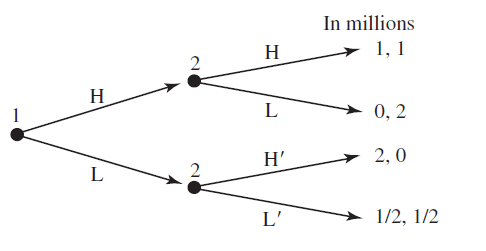
\includegraphics[width=0.8\textwidth]{7.f2_7}
\label{fig:f2_7}}
\vspace{2mm}
\end{center}

Let $s_i$ denotes a single strategy of player $i$,

There are 2 strategies for player 1: $s_1 =H$ and $s_1=L$. 

There are 4 strategies for player 2 : $s_2 =HH'$, $s_2 =HL'$, $s_2 =LH'$, and $s_2 =LL'$.

\begin{itemize}
\item $H$ and $H'$ are the same choice for player 2, but under 2 different conditions (how player 1 moves).
\item $HH'$ means "when player 1 chooses $H$, player 2 chooses $H$; when player 1 chooses $L$, player 2 also chooses $H$". 
\item We use $H'$ instead of $H$ just to distinguish the two conditions.
\end{itemize}

Player 2's strategy has a form of ``$s_2 = [s_2(s_1 = H),s_2(s_1 = L)]$'', where $s_2(s_1 = H)$ can be either $H$ or $L$, and $s_2(s_1 = L)$ can be either $H'$ or $L'$. There are $2 \times 2 = 4$ different strategies.

\vspace{3mm}

Now think, in the pizza problem:

\end{mdframed}

Both player 1 and player 2 have 9 different choices, and player 1 moves first.
Player 2's strategy is:

$[s_2(s_1 = 0), s_2(s_1 = 1), s_2(s_1 = 2), s_2(s_1 = 3), s_2(s_1 = 4), s_2(s_1 = 5),
 \\ s_2(s_1 = 6), s_2(s_1 = 7), s_2(s_1 = 8)]$

where each $s_2(s_1 = n)$ can take 9 values in $[0,8]$ ($9^9$ strategies in total).


\begin{mdframed}[backgroundcolor=blue!20,linecolor=white]
This seems redundant but it's necessary to represent all the information, which is critical for an equilibrium. See question \ref{subsec:ne}.

\medskip 

Here is another example to show the problem more clearly.


\begin{center}
{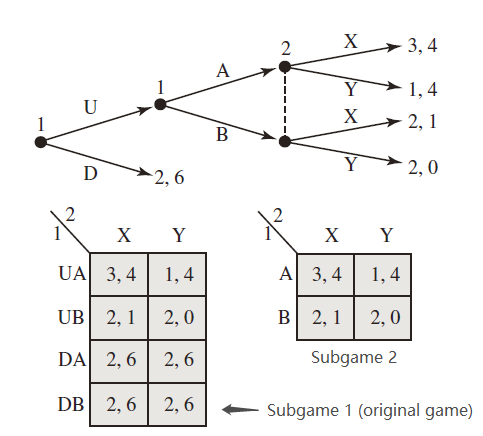
\includegraphics[width=0.8\textwidth]{7.f15_4}
\label{fig:f15_4}}
\vspace{2mm}
\end{center}

\textbf{Strategy Set/Space} (Watson pp.23)

We use $S_i$ to denote the strategy set/space for player $i$ (a set comprising each of the possible strategies of player $i$ in the game).

\medskip 

In the original game, player 1 has 4 single strategies. The strategy space $S_1 = \{UA,UB,DA,DB\}$; while player 2 only has 2 strategies, $S_2 = \{X,Y\}$.

\begin{itemize}
\item The number of strategies depends on how many decisions (information set) player i has to make.
\item Nodes linked by a dashed line is ONE information set (player 2 can't know if player 1 chooses A or B, therefore he/she can make one decision, $X$ or $Y$.)

\end{itemize}

\end{mdframed}


%
%***************************************************
\subsection{Find all the pure-strategy Nash equilibrium outcomes. }
\label{subsec:ne}

\begin{mdframed}[backgroundcolor=blue!20,linecolor=white]

\textbf{Subquesiton \ref{subsec:ne} and Subquesiton \ref{subsec:spne} are to help you
understand why we need to refine NE to SPNE for a dynamic game.}
\medskip

A NE is a state in which nobody can improve his/her payoff by deviating from his/her own strategy unilaterally.

\smallskip

To ahcieve a NE, player 2 must have his/her best response against $s_1$, and also make sure player 1 will not regret choosing $s_1$ (then deviate).

\medskip

Actually, we already found all the static NE for in Table \ref{tab:pizza}, what we need to do is to "rewrite" them in a dynamic way s.t. no one will deviate.

\smallskip

Take a NE $(2,6)$ in Table \ref{tab:pizza} for example.

\begin{itemize}
\item When player 1 chooses 2 first, the best response for player 2 is to choose 6;
\item To make sure player 1 will not deviate from choosing 2, player 1 must "eliminate" player 1's incentive to deviate, i.e. let $u_1(s_1=2,s_2) \ge u_1(s_1 \ne 2,s_2)$.
\item A strategy $s_2$ such as $(4,8,\textcolor{red}{6},6,5,4,3,2,1)$ achieves such a NE. 
\item Note the red \textcolor{red}{6} is the outcome (payoff) but not a "strategy". A strategy is a complete contingent plan. Here includes both the result player 2 wants (\textcolor{red}{6}) and the threat part ("if you choose less than 2, fine; if you choose more than 2, I'll let you have nothing").
\end{itemize}

We find $(2,(4,8,\textcolor{red}{6},6,5,4,3,2,1))$ is a dynamic NE.
\medskip

For all the NE (except $(8,8)$) found in Table \ref{tab:pizza}, we can express them as:
\smallskip

$$s^\ast_1 \in \{0,1,2,3,4,5,6,7,8\} \ \ \  and$$ 
$$s^\ast_2(s_1) = 8 - s_1 \ \ if \ \ s_1 = s^\ast_1$$
$$s^\ast_2(s_1) > 8 - s_1 \ \  if \ \ s_1 > s^\ast_1$$
$$s^\ast_2(s_1) \in \{0,1,2,3,4,5,6,7,8\}\ \  if \ \ s_1 < s^\ast_1$$

The static NE $(8,8)$ is a little different to rewrite, but the idea is the same.
\begin{itemize}
\item When player 1 chooses 8 first, any natural number in $[0,8]$ is a best response of player 2. Thus 8 is one of the best responses of player 2.
\item To make sure player 1 not deviating, player 2 must ruin player 1's incentive again. "If you don't choose 8, you get nothing either, then why deviate?"
\end{itemize}

$$s^\ast_1 = 8 \ \ \ \ and$$ 
$$s^\ast_2(s_1) > 8 - s_1 \ \ if  \ \ s_1 \in \{1,2,3,4,5,6,7,8\}$$
$$s^\ast_2(s_1) \in \{0,1,2,3,4,5,6,7,8\} \ \ if  \ \ s_1 = 0$$

To conclude, the static NE is exactly the payoff outcome of the dynamic NE. 
Dynamic NE are strategies that keep static NE stable.
\end{mdframed}


(1) Type 1:

$s^\ast_1 \in \{0,1,2,3,4,5,6,7,8\}$ and \\
$s^\ast_2(s_1) = 8 - s_1$ if $s_1 = s^\ast_1$, \\
$s^\ast_2(s_1) > 8 - s_1$ if $s_1 > s^\ast_1$, \\
$s^\ast_2(s_1) \in \{0,1,2,3,4,5,6,7,8\}$ if $s_1 < s^\ast_1$. \\

\begin{mdframed}[backgroundcolor=blue!20,linecolor=white]
\textit{Example:} $(4, (8,7,6,5,4,4,4,4,4))$

Here player 2 demands the pieces that are left if player 1 does not demand more than 4 pieces, but demands 4 pieces if player 1 demands more than 4 pieces. 
To demand 4 pieces is a best response for player 1, given that he will not get anything if demands more than 4 pieces.
It is a best response for player 2, given that player 1 demands 4 pieces, as his strategy specifies.
\end{mdframed}


(2) Type 2:

$s^\ast_1 = 8$ and \\
$s^\ast_2(s_1) > 8 - s_1$ if $s_1 \in \{1,2,3,4,5,6,7,8\}$, \\
$s^\ast_2(s_1) \in \{0,1,2,3,4,5,6,7,8\}$ if $s_1 = 0$.

\begin{mdframed}[backgroundcolor=blue!20,linecolor=white]
\textit{Example:} $(8, (8,8,8,8,8,8,8,8,8))$

Here player 2 demands all the 8 pieces independently of what player 1 demands. 
To demand all the 8 pieces is a best response for player 1, given that he will not get anything anyway. 
It is a best response for player 2, given that player 1 demands all the 8 pieces, as his strategy specifies.

\end{mdframed}

%
%***************************************************
\subsection{Find all the pure-strategy subgame perfect equilibria.}
\label{subsec:spne}

\begin{mdframed}[backgroundcolor=blue!20,linecolor=white]

The NE found in Subquestion \ref{subsec:spne} sound good, but is player 2's threat like "if you choose more than 2, I'll let you have nothing" valid? 

\begin{itemize}
\item If player 1 chooses 7, and the game is played only once, what will player 2 do to maximize  utility (BR)?
\item "To give in and accept the 1 piece pizza left by player 1" is BR for player 2.
\end{itemize}

NE is an ex ante view of the game. But in a dynamic game, players need to think "if something already happened, what should I do", which is an ex post view.

\medskip

\textbf{Sequential rationality} (Watson pp.186): An optimal strategy for a player should maximize
his or her expected payoff, conditional on every information set
at which this player has the move. That is, player i’s strategy should
specify an optimal action from each of player i’s information sets, even
those that player i does not believe (ex ante) will be reached in the game.

\medskip

\textbf{SPNE} (Watson pp.189): A strategy profile is called a subgame perfect Nash equilibrium (SPNE) if it specifies a Nash equilibrium in every subgame of the original game.

\begin{itemize}
\item  SPE is a NE
\item  For games of perfect information,  backward induction yields subgame perfect equilibria(Watson pp.191).
\item  For games of imperfect information, we need to check every subgame (Read Watson pp.190).
\end{itemize}

Here is an example of extensive form when player 1 chooses 3 and 7 (I didn't draw the 
whole extensive form because it takes too much space).

\tikzstyle{solid node}=[circle,draw,inner sep=1.5,fill=black]
\begin{tikzpicture}
\node(0)[solid node,label=left:{Player 1 chooses 3}]{}
[grow=east]
  child{node[solid node,label=right:{$(0,0)$}]{} edge from parent node[below]{8} }
  child{node[solid node,label=right:{$(0,0)$}]{} edge from parent node[below]{7} }
  child{node[solid node,label=right:{$(0,0)$}]{} edge from parent node[below]{6} }
  child{node[solid node, red, label=right:{$(3,5)$}]{} edge from parent[red] node[below]{5} }
  child{node[solid node,label=right:{$(3,4)$}]{} edge from parent node[below]{4} }
  child{node[solid node,label=right:{$(3,3)$}]{} edge from parent node[below]{3} }
  child{node[solid node,label=right:{$(3,2)$}]{} edge from parent node[below]{2} }
  child{node[solid node,label=right:{$(3,1)$}]{} edge from parent node[below]{1} }
  child{node[solid node,label=right:{$(3,0)$}]{} edge from parent node[below]{0} }
;
\end{tikzpicture}
\captionof{figure}{When player 1 chooses 3}
\label{fig:s_1=3}

\begin{tikzpicture}
\node(0)[solid node,label=left:{Player 1 chooses 7}]{}
[grow=east]
  child{node[solid node,label=right:{$(0,0)$}]{} edge from parent node[below]{8} }
  child{node[solid node,label=right:{$(0,0)$}]{} edge from parent node[below]{7} }
  child{node[solid node,label=right:{$(0,0)$}]{} edge from parent node[below]{6} }
  child{node[solid node,label=right:{$(0,0)$}]{} edge from parent node[below]{5} }
  child{node[solid node,label=right:{$(0,0)$}]{} edge from parent node[below]{4} }
  child{node[solid node,label=right:{$(0,0)$}]{} edge from parent node[below]{3} }
  child{node[solid node,label=right:{$(0,0)$}]{} edge from parent node[below]{2} }
  child{node[solid node, red, label=right:{$(7,1)$}]{} edge from parent[red] node[below]{1} }
  child{node[solid node,label=right:{$(7,0)$}]{} edge from parent node[below]{0} }
;
\end{tikzpicture}
\captionof{table}{When player 1 chooses 7}
\label{fig:s_1=7}

\medskip

With backward induction, we can find when player 1 chooses 7, player 2 will accept 1.
Therefore player 1 will never choose less than 7. 

\smallskip

Then how about player 1 chooses 8? In this case, player 2 get nothing, no matter what he/she chooses. But on the other hand, player 2 can freely (there is nothing to lose, anyway) choose any pieces more than 0 to punish the greedy player 2 (ruin everything). 

As a result, we have SPNE:

$$(7,(8,7,6,5,4,3,2,1,n)), \ n \in \{1,2,3,4,5,6,7,8\}$$

However, if player 2 doesn't decide to punish player 1 (maybe they don't want the restaurant owner to have the pizza back), there can still be a SPNE:

$$(8, (8,7,6,5,4,3,2,1,0))$$

The two types of SPNE results from the fact that player 2's payoff is 0 (and then indifferent to any choices) whenever player 1 chooses 8. 

\end{mdframed}

(1) Type 1:

$s^\ast_1 = 7$ and \\
$s^\ast_2(s_1) = 8 - s_1$ if $s_1 \in \{0,1,2,3,4,5,6,7\}$, \\
$s^\ast_2(s_1) > 8 - s_1$ if $s_1 = 8$. \\

\begin{mdframed}[backgroundcolor=blue!20,linecolor=white]
Example: $(7, (8,7,6,5,4,3,2,1,1))$ 

Here player 2 demands the pieces that are left if player 1 demands less that all the 8 pieces, but demands 1 piece if player 1 demands all 8 pieces. This is a best response for player 2, not only if player 1 demands 7 pieces, as his strategy specifies, but also for all other choices that player 1 might do. To demand 7 pieces is a best response for player 1, given that he will not get anything if he demands all the 8 pieces.

\end{mdframed}


(2) Type 2:

$s^\ast_1 = 8$ and \\
$s^\ast_2(s_1) = 8 - s_1$ if $s_1 \in \{0,1,2,3,4,5,6,7,8\}$ 

That is: $(8, (8,7,6,5,4,3,2,1,0))$

\begin{mdframed}[backgroundcolor=blue!20,linecolor=white]
Here player 2 requires the pieces that are left. This is a best response for player 2, not only if player 1 demands all the 8 pieces, as his strategy specifies, but also for all other choices that player 1 might do. To demand all the 8 pieces is a best response for player 1.
\end{mdframed}

%


\vspace{-6pt}

\bigskip

%%%%%%%%%%%%%%%%%%%%%%%%%%%%%%%%%%%%%%%%%%%%%%%%%%%%%%%%%%%%%%%%%%%%%%%%%%%%%%%%%%%%%%%%%%%%%%
\newpage

\section{Problem 2 - Best response sets} 

Exercise 6.4 

For the game of Figure 6.2 (Watson pp.55), determine the following best-response sets.


{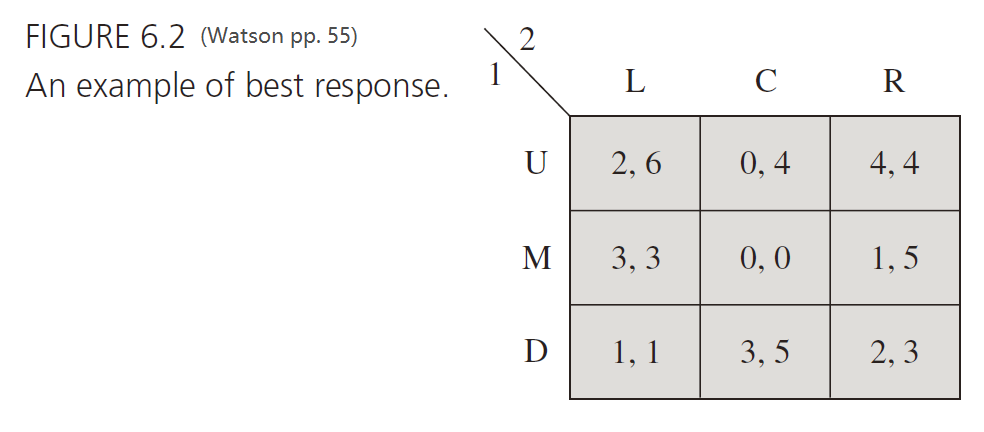
\includegraphics[width=0.8\textwidth]{7.f6_2}
\label{fig:f6_2}}
\vspace{2mm}

%***************************************************

\begin{mdframed}[backgroundcolor=blue!20,linecolor=white]

\textbf{(a) $BR_1(\theta_2)$ for $\theta_2 = (1/6,1/3,1/2)$}

$$U^1_U(\theta_2) = \frac{1}{6} \times 2 + \frac{1}{3} \times 0 + \frac{1}{2}\times 4=\frac{14}{6}$$
$$U^1_M(\theta_2) = \frac{1}{6} \times 3 + \frac{1}{3} \times 0 + \frac{1}{2}\times 1=1$$
$$U^1_D(\theta_2) = \frac{1}{6} \times 1 + \frac{1}{3} \times 3 + \frac{1}{2}\times 2=\frac{13}{6}$$

$BR_1(\theta_2)=\{U\}$

\medskip

\textbf{(b) $BR_2(\theta_1)$ for $\theta_1 = (1/6,1/3,1/2)$}

$$U^2_L(\theta_1) = \frac{1}{6} \times 6 + \frac{1}{3} \times 3 + \frac{1}{2}\times 1=2.5$$
$$U^2_C(\theta_1) = \frac{1}{6} \times 4 + \frac{1}{3} \times 0 + \frac{1}{2}\times 5=2.5 + \frac{2}{3}$$
$$U^2_R(\theta_1) = \frac{1}{6} \times 4 + \frac{1}{3} \times 5 + \frac{1}{2}\times 3=2.5 + \frac{4}{3}$$

$BR_2(\theta_1)=\{R\}$

You just keep doing this...
\end{mdframed}

(a) $\{U\}$ \\ \indent (b) $\{R\}$ \\ \indent (c) $\{U\}$ \\ \indent (d) $\{U,D\}$ \\ \indent (e) $\{L,R\}$

\bigskip

\section{Problem 3 - BR functions, NE, rationalizable strategies}

(Watson Exercise 9.6 )

Consider a game in which, simultaneously, player 1 selects any real number
$x$ and player 2 selects any real number $y$. The payoffs are given by:
$$u_1(x,y)= 2x-x^2+2xy$$
$$u_2(x,y)= 10y-2xy -y^2$$

%***************************************************
\subsection{Calculate and graph each player's best-response function as a function
of the opposing player’s pure strategy.}

\begin{mdframed}[backgroundcolor=blue!20,linecolor=white]
Given any y, how can player $1$ maximize his/her utility? FOC and SOC!
\end{mdframed}

\textbf{For player 1:}
\medskip
FOC:
$$\frac{d u_1(x,y)}{d x} = \frac{d 2x-x^2+2xy}{d x} = 2 - 2x +2y =0 \Rightarrow x = 1+y$$
SOC: 
$$\frac{d^2 u_1(x,y)}{d x^2} = -2<0$$

Therefore  $BR_1(y) = 1+y$

\medskip

\textbf{For player 2:}
\medskip
FOC:
$$\frac{d u_2(x,y)}{d y} = \frac{d  10y-2xy -y^2}{d y} = 10-2x-2y =0 \Rightarrow y = 5-x$$
SOC: 
$$\frac{d^2 u_2(x,y)}{d y^2} = -2<0$$

Therefore  $BR_2(x) = 5-x$

\begin{center}
\begin{tikzpicture}[scale = 0.9]
\draw[thick,<->] (0,8) node[left]{$y$}--(0,0)--(8,0) node[right]{$x$};
\draw[thick] (-2.5,0) --(0,0)--(0,-3.5);
\node [below left] at (0,0) {$0$};

\draw [red] (-2,7)--(7,-2)node[right]{$BR_2(x)$};
\draw [blue] (-2,-3)--(6,5)node[right]{$BR_1(y)$} ;

\node[left] at (0,5) {$5$} ;
\node[below] at (5,0) {$5$} ;
\node[left] at (0,-1) {$-1$} ;
\node[below] at (1,0) {$1$} ;
\node[below] at (3,0) {$3$} ;
\node[left] at (0,2) {$2$} ;

\draw [dashed] (0,2)--(3,2)node[right]{$NE={(3,2)}$};
\draw [dashed] (3,0)--(3,2);

\end{tikzpicture}
\captionof{figure}{$BR_1(y)$ and $BR_2(x)$}
\label{fig:br}
\end{center}
\vspace{2mm}

%***************************************************
\subsection{Find and report the Nash equilibria of the game.}

$NE(x^*,y^*)$ is a point s.t. $BR_1(y^*) = x^*$ and $BR_2(x^*)=y^*$, thus

$$x^* = 1+y^*$$
$$y^* = 5-x^*$$
(2 functions, 2 variables, we can solve $x^*,y^*$)

$\Rightarrow x^*= 3, y^*=2 \ \Rightarrow \ NE=(3,2)$

%***************************************************
\subsection{Determine the rationalizable strategy profiles for this game.}

\begin{mdframed}[backgroundcolor=blue!20,linecolor=white]

\textbf{rationalizable strategies}(Watson pp.70): The set of strategies that
survive iterated dominance is therefore called the rationalizable strategies.

\textbf{Dominance}(Watson pp.50): A pure strategy $s_i$ of player $i$ is dominated if there is a strategy (\textbf{pure or mixed}) $\sigma_i \in \Delta S_i$ such that $u_i(\sigma_i , s_{-i}) > u_i (s_i , s_{-i})$, for all strategy profiles $s_{-i} \in S_{-i}$ of the other players.

\end{mdframed}

\begin{itemize}
\item Since $BR_1(y) = 1+y$, all the numbers in $(-\infty,+\infty)$ can be the best response of player 1 sometimes;
\item Since $BR_2(x) = 5-x$, all the numbers  in $(-\infty,+\infty)$ can be the best response of player 2 sometimes too.

\end{itemize}

Therefore there is no dominated strategy (a number that can never be BR) for the two players.

The set of rationalizable strategies is $(-\infty, +\infty) \times (-\infty, +\infty) = (-\infty, +\infty)$.

\begin{mdframed}[backgroundcolor=blue!20,linecolor=white]
Note the symbol ``$\times$'' denotes the Cartesian product here. For example, if $S_1={A,B}, S_2={X,Y}$,then $$S= S_1 \times S_2 = {(A,X),(A,Y),(B,X),(B,Y)}$$
\end{mdframed}


\bigskip

\section{Problem 4 - True or False?}

For each of the statements, if true, try to explain why, and if false, provide a
counter-example.

\begin{itemize}
%
\item[(a)] In a finite extensive-form game of perfect information, there always exists a subgame perfect Nash equilibrium. 

\medskip

True(Watson pp.188). A subgame-perfect Nash equilibrium can be constructed by using backward induction.

\begin{mdframed}[backgroundcolor=blue!20,linecolor=white]
A more detailed explanation is on Jehle \& Reny pp.317 : every finite extensive-form game possesses at least one NE.
\end{mdframed}

\item[(b)] In a finite extensive-form game of perfect information, there always exists a unique subgame perfect Nash equilibrium.  
\medskip

False. The pizza game is a complex counter-example. Here is another:

\end{itemize}

\begin{center}
\tikzstyle{solid node}=[circle,draw,inner sep=1.5,fill=black]
\begin{tikzpicture}
\node(0)[solid node,label=left:{P1}]{}
[grow=east]
  child{node(1)[solid node,label=below:{P2}]{}
    child{node(2)[solid node,label=right:{$(0,2)$}]{} edge from parent node[below]{b}}
    child{node(2)[solid node,label=right:{$(2,2)$}]{} edge from parent node[above]{a}}
    edge from parent node[below,xshift=-3]{in}}
  child{node(1)[solid node,label=right:{$(1,1)$}]{} edge from parent node[above,xshift=-3]{out}};
\end{tikzpicture}
\captionof{figure}{Counter-example}
\label{fig:example}
\end{center}

When player 2 is \textbf{indifferent}(recall the pizza game) to $a$ and $b$, there can be many SPNE:

$$(out,(b,b)),(out,(a,b)),(in,(b,a)),(in,(a,a))$$

Here $(a,b)$ means $s_2(out)=a, s_2(in)=b$.


\section{Problem 5- Firm-union bargaining}

A firm's output is $L(100-L)$ when it uses $L \leq 50$ units of labor, and $2500$ when it uses
$L \geq 50$ units of labor. The price of output is $1$. A union that represents workers
presents a wage demand (a nonnegative number $w$), which the firm either accepts or rejects. If
the firm accepts the demand, it chooses the number $L$ of workers to employ (which you should
take to be a continuous variable, not an integer); if it rejects the demand, no production
takes place ($L = 0$). The firm's preferences are represented by its profits, the union's
preferences are represented by  the value of $wL$.

%***************************************************
\subsection{Formulate this situation as an extensive game with perfect information. }

\textbf{Players}: $N = \{U, F \}$. \\ 
\textbf{Strategies}: 
\begin{itemize}
\item $U$ chooses a wage $w$ from the set of non-negative number; 
\item $F$ chooses a function that to any non-negative wage $w$ determines a non-negative employment $L(w)$.
\end{itemize}

\textbf{Payoffs}: 

\begin{itemize}
\item The union's payoff is $U^U(L,w)=wL(w)$; 
\item The firm's payoff is 
\begin{itemize}
\item $U^L(L,w)=L(w)(100-L(w)) - wL(w)$ if $L(w) \le 50$
\item $U^L(L,w)=2500 - wL(w)$ if $L(w) \ge 50$
\end{itemize}

\end{itemize}

Note $L(w) = 0$ is in effect a rejection by the firm of the demand $w$, giving both a payoff of $0$.
%
%***************************************************
\subsection{Find the subgame perfect equilibrium (equilibria?) of the game.}

(1) Given any wage $w$, the firm wants to maximize its profit. 

FOC:
$$\frac{d U^L(L,w)}{d L} = \frac{d L(w)(100-L(w)) - wL(w)}{d L} = 100-2L-w =0 \Rightarrow L(w) = 50-0.5w$$
SOC: 
$$\frac{d^2 U^L(L,w)}{d L^2} = -2<0$$

(2) The union realizes the firm's best response, and maximizes its utility according to it:
$$\max_{w} U^U(w) = w (50-0.5w)$$

FOC:
$$\frac{d U^U(w)}{d w} = \frac{d w (50-0.5w)}{d w} = 50-w =0 \Rightarrow w = 50$$
SOC: 
$$\frac{d^2 U^U(L,w)}{d L^2} = -1<0$$

When $w=50$, $L(50)=50-0.5\times50 =25$


SPNE: $(w= 50,50-0.5\times w)$

%
%***************************************************
\subsection{Is there an outcome of the game that both parties prefer to any subgame perfect
equilibrium outcome? }

\begin{mdframed}[backgroundcolor=blue!20,linecolor=white]
"An outcome that both parties prefer to any SPNE outcome" means Pareto improvement exists.

\medskip

For this kind of welfare problem, think what will happen if you're a ``social planner", i.e. you can allocate resources freely between $F$ and $U$, and what you care is the joint surplus $U^T=U^F+U^U$.

\end{mdframed}

$$U^T=U^F+U^U = L(100-L) - wL +wL =L(100-L)$$

FOC:
$$\frac{d U^T(L)}{d L} = \frac{d L(100-L)}{d L} = 100-2L =0 \Rightarrow L = 50$$
SOC: 
$$\frac{d^2 U^T(L)}{d L^2} = -2<0$$

Therefor $U^T_{max} = 50 (100-50) =2500$.

\medskip

Compare with SPNE $(w= 50,50-0.5\times w)$:

$$U^F_{SPNE} = 25(100-25)-50\times 25 = 625$$
$$U^U_{SPNE} = 50 \times 25 = 1250$$
$$U^T_{SPNE} = 625 + 1250 = 1875$$

\begin{mdframed}[backgroundcolor=blue!20,linecolor=white]

Obviously, if the firm cooperates with the union, the joint surplus is more than the one in SPNE.

\medskip

Now let's check if it's possible to allocate $U^T_{max} = 2500$ between the firm and the union s.t. at least one player's welfare is more than SPNE outcome, without harming the other player (Pareto improvement).

\end{mdframed}

\medskip

(1) If we keep the firm intact ($U$ benefits the most), i.e. let $U^F = U^F_{SPNE} = 625$,
we have $U^U=U^T-U^F = 2500-625 = 1875$ left for the union, i.e. $U^U = 1875$.
The wage $w= \frac{U^U = 1875}{50}=37.5$;

\medskip

(2) If we keep the union intact ($F$ benefits the most), i.e. let $U^U = U^U_{SPNE} = 1250$,
Given $L = 50$, the wage $w= \frac{U^U = 1250}{50}=25$; Now
we have $U^F =U^T-U^U = 2500-1250 = 1250$ left for the firm.

\medskip

Actually, at this employment level ($L=50$), any wage $w \in [25,37.5]$ would lead to a Pareto-improvement. 
%
%***************************************************
\subsection{Find a Nash equilibrium for which the outcome differs from any subgame perfect
equilbrium outcome.}

\begin{mdframed}[backgroundcolor=blue!20,linecolor=white]
SPNE are NE without "empty threat". To find a NE different from SPME, we can start by making an empty threat.

\end{mdframed}

Now the firm makes a threat on low wage, "refuse to hire anyone if $w > 20$", i.e.:

\begin{equation}
L(w)=
    \begin{cases}
    50-0.5w \ \ if \ \ w \le 20 \\
    0 \ \ if \ \ w > 20 \\
    \end{cases}
    \label{eq:threat}   
\end{equation}

For such a threat, the union's BR is to accept $w=20$. 
Note also $L = 50-0.5w$ is the BR of the firm. Then both of the two players will not deviate.

($w=20$, the threat above) is a NE but not a SPNE.




\end{document}